\subsection*{Tokamak and Tokamak Plasma Structure}
    Consider now the structure of a tokamak, and with it the structure of the plasma contained within. Most crucially, the chamber is (approximately) rotationally symmetric in the vertical axis. Tokamak chambers are (almost always) \emph{almost} toroidal in topology, albeit for the presence of divertors on the reactor wall: specialized regions where the plasma is directed away from the interior, allowing for the removal of impurities and heat.
    
    As a result of Alfvén's frozen-in flux theorem \cite{Alfvén_1943}, the plasma dynamics within the chamber are largely guided by the shape of the magnetic field (up to particle drifts) particularly in the ideal limit, as the plasma is ``tied'' to the magnetic field lines. One can therefore gain an understanding of the structure of the plasma within a tokamak by looking at the structure of the magnetic fields. (See Figure \ref{fig:tokamak structure}) The magnetic field within a tokamak has two components:
    \begin{itemize}
        \item  {\bf The toroidal field:} Generated by magnetic coils perpendicular to the length of the tokamak (parallel to the cross section in the diagram) and directed around the length of the tokamak (into the diagram).
        \item  {\bf The poloidal field:} Generated by magnetic coils around the length of the tokamak (into the diagram) and directed perpendicular to the toroidal field (parallel to the cross section in the diagram).
    \end{itemize}
    The combination of these two magnetic fields creates ``flux surfaces'': 2D surfaces created by extending the magnetic field lines around the torus, within which the plasma is confined (labelled as ``closed magnetic surfaces'' and ``open magnetic surfaces'' in Figure \ref{fig:tokamak structure}). Many ``local'' models consider the plasma dynamics just along these flux surfaces.

    \begin{figure}[!ht]
        \centering
        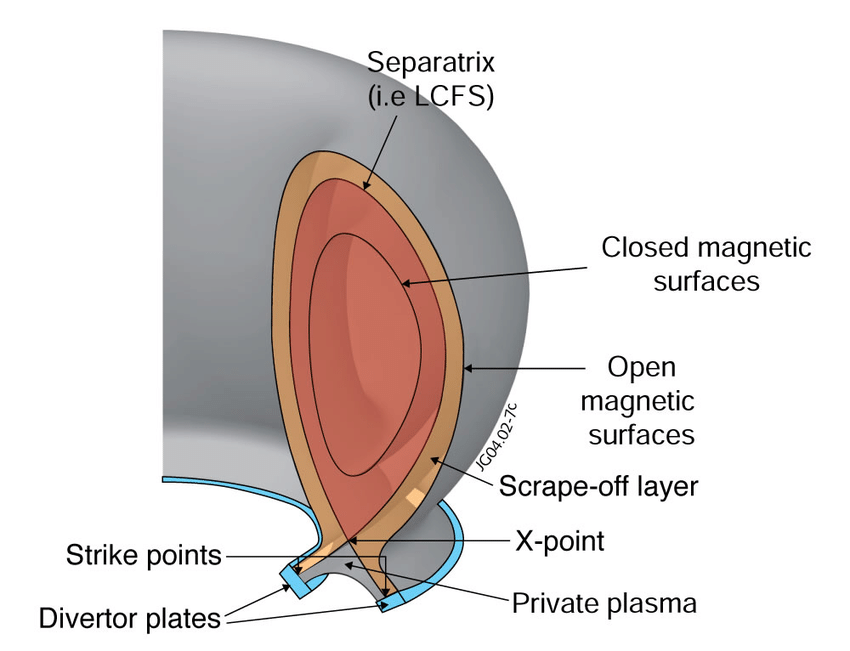
\includegraphics[width = 0.8\textwidth]{1 - plasmas/3 - tokamaks/images/tokamak structure.png}
        \caption{Cross-sectional diagram showing the magnetic field structure within a tokamak. (Source: European Fusion Development Agreement (EFDA))}
        \label{fig:tokamak structure}
    \end{figure}

    The structure of these flux surfaces divide the tokamak plasma into several distinct regions, each with its own properties:
    \begin{itemize}
        \item  {\bf The core and edge regions:} The central regions of the plasma, where the flux surfaces are \emph{closed} such that the plasma is fully contained. The core represents the center of this region, where the temperature and density are highest and the plasma is its most stable, and it is here where the majority of the fusion reactions occur.
        \item  {\bf The scrape-off layer (SOL) and divertor region:} Between the edge of the plasma and the tokamak walls, where the flux surfaces are \emph{open} such that the plasma is diverted into a divertor. This is separated from the edge plasma by a flux surface called the ``separatrix'', or ``last closed flux surface'' (LCFS). This is referred to as the divertor region when it enters a divertor, allowing for the removal of impurities and heat.
        \item  {\bf Private plasmas:} The small regions of the plasma contained around divertor, that do not form part of the SOL/divertor region.
    \end{itemize}
    The strength of the magnetic field and the shape of the flux surfaces can be controlled to optimize the confinement of the plasma and achieve the conditions necessary for fusion.
    